\section{VIA Relay Selection}
\label{sec:via:design}

Having shown that relaying through \hybrid could provide significant gains, 
we now devise a {\em practical} algorithm for relay selection. 
%In this section, we focus on the design of \hybrid's relay selection algorithm. 
 We begin by formulating the problem of relay selection. We describe 
 two classes of strawman approaches --- purely {\em predictive} and {\em exploration-based} ---
 and highlight limitations of both classes. We then present
 the core intuition behind our relay selection algorithm, called {\em prediction-guided exploration} and then describe 
 the solution. 

 
\subsection{Problem Formulation} 

Our goal  is to assign each call  to a particular \option as discussed in
Section~\ref{sec:via:arch}.  Recall that a \option can use the \direct
path, use a specific one-hop relay node (i.e., bouncing relaying), or use a specific pair of 
relay nodes (i.e., transit relaying).  Let  $\CallSet$ denote the set of calls we want to 
optimize and  let $\RelaySet$ denote the set of available \options. 
 We use $\Call \in \CallSet$ and   $\Relay \in
\RelaySet$ to denote a specific call and \option, respectively.
 Let $\QualityFunc(\Call, \Relay)$ denote the expected  
 {value of a network metric for} $\Call$  when using $\Relay$ {(a smaller value is better)}.
We assume that the relaying decisions for calls are independent; i.e., the performance of a call is not impacted by the relaying decisions made for other calls.

%We assume that the \hybrid framework has as input a a set of observed call records with
%measured performance metrics, $\HistoryCallSet$. Given $\HistoryCallSet$, 

The
goal of \hybrid is to  {\em assign} optimal \options
 for each $\Call \in \CallSet$. Let $\Assign:\CallSet \rightarrow \RelaySet$ denote 
 the assignment function output by some algorithm and 
 let $\Assign(\Call)$ be the \option assigned for call $\Call\in\CallSet$.
 Formally, our objective is to find  the optimal 
 assignment
 
\begin{displaymath}\arg\min_{\Assign \in \RelaySet^\CallSet}  \sum_{\Call\in\CallSet}\QualityFunc(\Call, \Assign(\Call))
\end{displaymath}

\noindent This is a minimization problem because a lower value is better for each of our network quality metrics $\QualityFunc$.

\subsection{Strawman Approaches}
\label{subsec:strawmen}

We can consider two classes of approaches for the optimal assignment of \options to calls:

\begin{enumerate}
%\vspace{-.05in}
\item  {\em Exploration-based:} One approach is to set aside a fraction of the 
 calls for measurement-based exploration of the performance of each possible relaying option for every source-destination pair.  
 For instance, for every AS-pair and every possible % one-hop/two-hop relaying, 
\option $\Relay$,
 we will explicitly use some of the calls to explore the option and measure the performance, 
  $\QualityFunc(\Call, \Relay)$.
  
%\vspace{-.05in}
\item  {\em Prediction-based:} An alternative to the exploration-based approach
 is to use the recent history  of observed call performance. Suppose, \hybrid has available as
 input  call records with measured performance $\HistoryCallSet$. Then, we can use
 suitable prediction algorithms  to 
 predict the performance $\QualityFunc(\Call, \Relay)$ for every combination, and select the option that has the best predicted performance.

\end{enumerate} 

Unfortunately, we observe in practice that both classes of approaches individually  have
very poor accuracy in predicting $\QualityFunc(\Call,
\Relay)$. This  ultimately results in a poor assignment strategy and poor call
quality.  There are two key reasons. 

First, there is  a fundamental problem because of {\em skew in data
density.} Specifically, there is a substantial difference in the number of
call samples available across different source-destination pairs, both for the
direct path and for the various relayed paths.  This variability arises because
of the large space of choices: $N$ end-points and $M$ relay strategies lead
to $O(N^2M)$ choices.  Furthermore, certain end-points make/receive
fewer calls, yielding fewer samples. Second, there is {\em inherent variability} in the observed performance.
Consequently, to estimate  $\QualityFunc(\Call, \Relay)$, we need  a
significant number of samples before the empirically observed values can
converge to the true values. 

The skew and the variability make prediction inaccurate and exploration ineffective and/or expensive (in terms of the effort to be expended).

%\sout{Note that these challenges have implications for both classes of approaches.  With 
% the prediction based approaches, skew implies that there will be some 
% coverage ``holes'' in the prediction-based approaches while the exploration-based 
% approaches may not have sufficient calls to explore all relay choices. \ga{Unclear.}
% Similarly, the noise induced by variability means that the prediction-based approaches
% can easily miss the optimal relaying strategy and the exploration-based approaches
% will need a substantial measurement budget to converge.} 


\begin{figure}[t!]
\centering
%\includegraphics[width=0.4\textwidth]{ppt-figs/Overview.png}
%\includegraphics[width=0.5\textwidth]{ppt-figs/Overview-new.pdf}
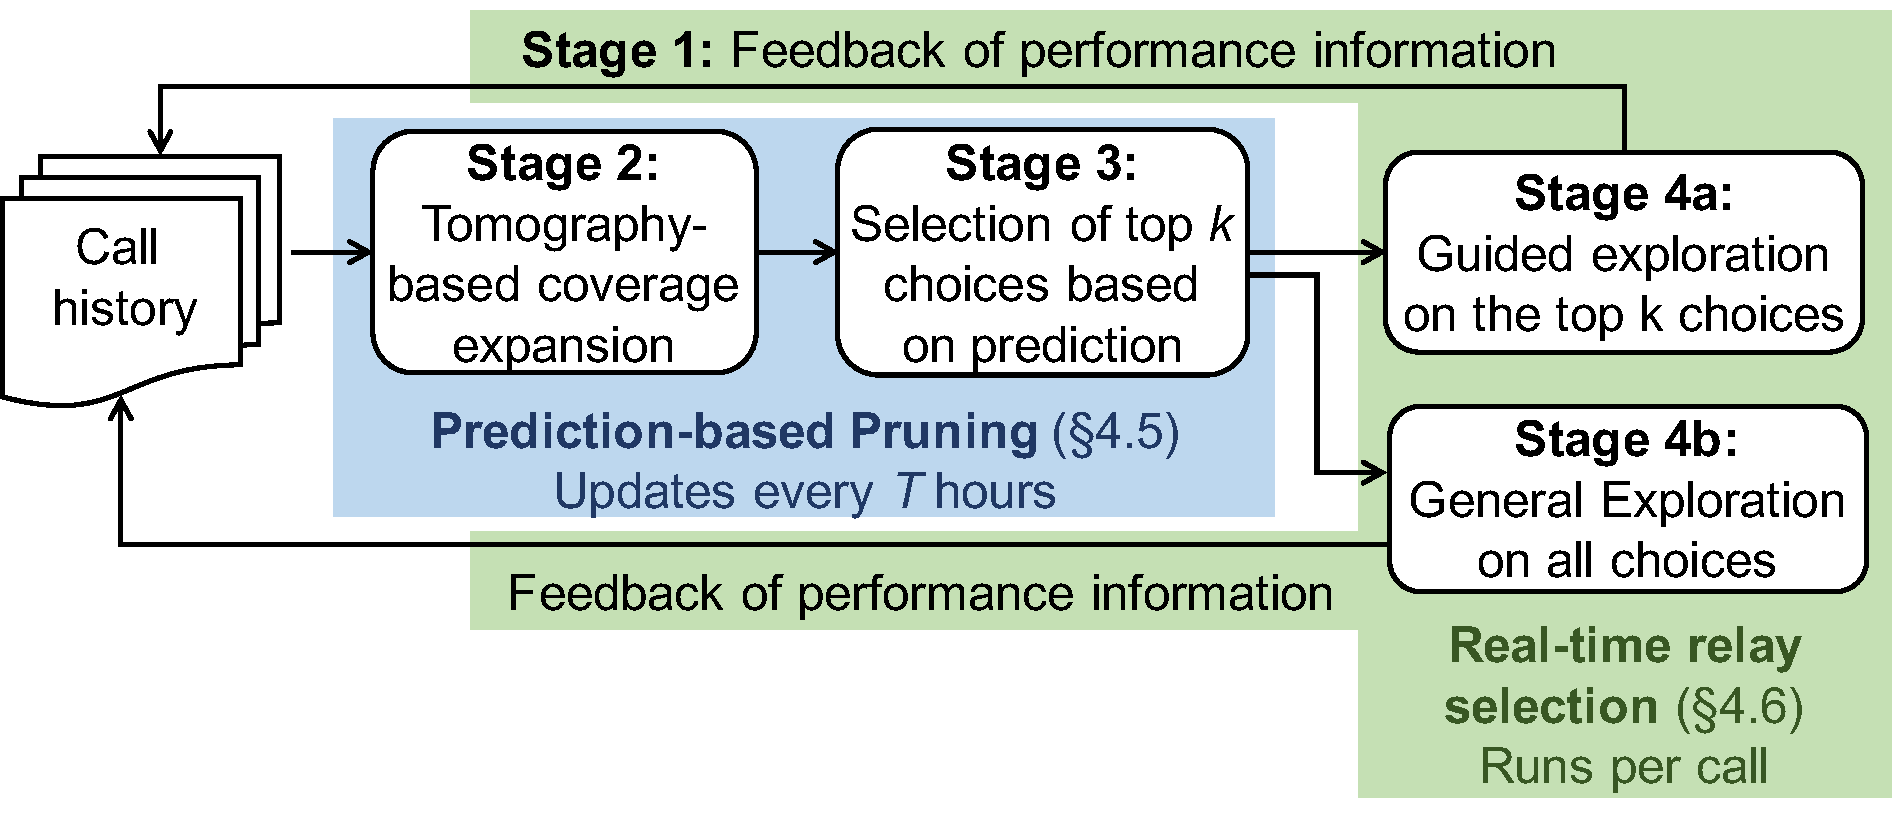
\includegraphics[width=0.5\textwidth]{figures/Via-Overview-new-ethan.pdf}
%\vspace{-0.5cm}
\caption{Overview of \hybrid relay selection based on prediction-guided exploration.}
\label{fig:intuition}
\end{figure}

%\subsection{Intuition behind our approach}
\subsection{Overview of \hybrid}
\label{subsec:Via-approach}

The key intuition behind our solution is the empirical observation that even though a prediction-based approach 
may not predict the optimal choice, the optimal is likely in the top few of its predictions. In other words, if we look at the top-$k$ choices 
(those who have the best predicted performances), the optimal choice will likely be a member of that set.%, even though it is a small subset of all possible \options $\RelaySet$. 
%may miss finding the true  optimal choice
%$\Relay^* = \arg\min_{\Relay \in RelaySet} \QualityFunc(\Call, \Relay)$, its
%prediction for that optimal choice 
%$\mathit{Prediction}(\QualityFunc(\Call, \Relay^*))$ is not too far away
%from the actual optimal value. A  natural corollary of  this observation is
%that if we look at a small number ($\leq 3$)   of top-k choices suggested by
%the prediction approach, then with high probability the true optimal strategy will be a member of
%that set; i.e., $\Relay^* \in \mathit{TopKPredictions}(\Call,k), k \leq 3$. 


We can exploit this observation to {\em prune} the search space for our
exploration  step. That is, the exploration approach does not need to blindly
explore the set   $\RelaySet$ of all possible strategies, but instead can focus
on a much smaller set of top-$k$ predictions.  We refer to this as a {\em
prediction-guided exploration}  approach.  
The top-$k$ pruning is not to be confused with a similar machine learning problem which seeks to find $k$ best options (e.g.,~\cite{cao2015top}). In contrast, we care more about the best \option {} -- our top-$k$ candidates may have bad options, but the best \option is very likely to be among them, and can be found by exploration techniques.

% Next, we describe the detailed design of the \hybrid approach
% for selecting the optimal relaying strategy. Algorithm~\ref{alg:hybrid} shows the psuedocode of \hybrid.


%\subsection{Overview of the \hybrid relay selection}
%\label{subsec:Via-approach}

Figure~\ref{fig:intuition} depicts the main stages in \hybrid, and Algorithm~\ref{alg:hybrid} shows the pseudocode. In a nutshell, the logical stages are: 
\begin{enumerate}
\item gathering performance information from call history, %\vspace{-.05in}
\item using network tomography to expand the coverage of the information from call history, %\vspace{-.05in}
\item using the (expanded) history information to predict performance and prune all but the most promising top-$k$ \options, and %\vspace{-.05in}
\item perform exploration-exploitation on the top-$k$ \options as well as all \options using multi-armed bandit (MAB) techniques.
\end{enumerate}

Finally, the observed performance of each call will be stored in call history, i.e., fed back to stage $1$.
Stages $2$ and $3$ (shown in light blue) %\vnp{the camera-ready paper will be in b\&w,so better to use a different method of highlighting} 
are performed at a periodicity of $T$ hours (by default $24$ hours), i.e., the pruned list of candidate \options are refreshed every $T$ hours.  Stages $1$ and $4$ (shown in light green) are performed on a per-call basis.
We discuss these stages in the sub-sections that follow.

\SetAlgoNoLine
\begin{algorithm}[t!]
\begin{small}
\nonl\hrulefill

\KwIn{Set of calls $\CallSet$ to be assigned to \options $\RelaySet$, and set of historical calls $\HistoryCallSet$}
\KwOut{A relay assignment, $\Assign$, where each call $\Call\in\CallSet$ is assigned a relay option $\Assign(\Call)\in\RelaySet$}

\nonl\hrulefill

%\red{Apply tomography to expand coverage of $\HistoryCallSet$}
\tcc{\scriptsize Stage 2: Tomography-based performance predictor trained from \HistoryCallSet}
$\Predictor\leftarrow \BuildPredictor(\HistoryCallSet)$

\tcc{\scriptsize Stage 3: Pick Top-$k$ candidates based on history-based prediction.}

$\Assign\leftarrow\emptyset$ 

\For{$(\Src,\Dst)$}{

	TopK$\leftarrow \GetTopK(\Src,\Dst,\RelaySet,\Predictor)$ 

	\tcc{\scriptsize See Algorithm~\ref{alg:pruning}}

	\For{$\Call\in\CallSet$}{

		\If{$RandomFloat(0,1) < \epsilon$}{
			\tcc{\scriptsize Stage 4a: Explore the Top-$k$ candidates}
			$\Relay\leftarrow\Explore(\Call,\Src,\Dst,\text{TopK},\Assign,\Predictor)$ 
		}\Else{
			\tcc{\scriptsize Stage 4b: Randomly explore all \options}
			$\Assign(\Call)\leftarrow Random(\RelaySet)$ 			
		}
		$\Assign(\Call)\leftarrow\Relay$ 
	}
}
\Return{\Assign} 

\nonl\hrulefill
\vspace{.1in}
\end{small}
\caption{\bf Relay selection algorithm of \hybrid}
\label{alg:hybrid}
\end{algorithm}


\subsection{Prediction-Based Pruning}
\label{subsec:practical-prediction}



% prediction, coverage vs. accuracy tradeoff
%The first step in \hybrid is to predict
Using call history data, \hybrid proceeds to predict, with confidence intervals, the performance between a source-destination pair over each \option:  direct paths, and each transit and  bouncing relay. %\vnp{"one-hop" and "two-hop" would be confusing, since it is actually 2 hops and 3 hops in the bouncing and transit cases, respectively} 

%\red{\noindent{\bf Expanding Coverage using Tomography:}
\mypara{Expanding coverage by network tomography}
Call history tells us the performance of paths that were actually used. 
As there is skew in call distribution, there might be ``holes'', i.e., no call history for the network path between a source-destination pair through a specific \option. 
Can we learn about the performance of these network paths? 
%Can we learn about the performance of network paths that are {\em not} contained in the history, e.g., one containing a relay not used before by a caller-callee pair? 

\begin{figure}[t!]
\centering
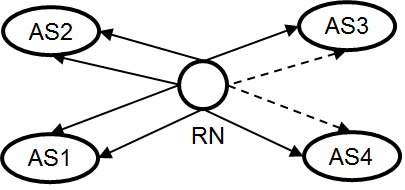
\includegraphics[width=0.4\textwidth]{figures/Via-Tomography.png}
\caption{Path stitching in \hybrid to estimate performance through relay RN. Solid lines represent historical call samples that we use to predict performance between AS$3$ and AS$4$ (dotted line). RTT$_{\text{AS3}\leftrightarrow\text{AS4}}$ $=$ RTT$_{\text{AS1}\leftrightarrow\text{AS4}}$ $+$ RTT$_{\text{AS2}\leftrightarrow\text{AS3}}$ $-$ RTT$_{\text{AS1}\leftrightarrow\text{AS2}}$.}
\label{fig:tomography}
\end{figure}

If we knew the performance of the individual network segments (e.g., client to relay) that comprise an end-to-end path, we could compose these to estimate the performance of the path. In principle, measurements of the individual network segments could be made by the relays themselves. However, the relays in \skype were only designed to forward traffic and we were not in a position to add new functionality to these relay nodes (and potentially impose additional overheads). 
%Nevertheless, how to leverage direct measurements between clients and relays, when they are available, is an area for future exploration.
%The situation is not unlike that in ISP networks where direct measurement of network links, while easy in principle, is challenging in practice, leading to indirect approaches for estimating such metrics as the link performance and the traffic matrix~\cite{tomo-gravity}.

 
Network tomography provides an alternative. By combining end-to-end measurements across several, partially-overlapping paths, network tomography can help estimate the performance of each network segment. Then, by stitching together the estimates for the individual segments, we can estimate the performance of a path not seen before.

Figure~\ref{fig:tomography} shows a simple example of how network tomography expands coverage. We use linear tomography, and apply it to individual 
%\cameraremove{which can be applied to }metrics that compose linearly (e.g., RTT) or can be linearized (e.g., jitter and packet loss rate, under the assumption of independence across network segments~\cite{Tomography-StatSci04}). 
%\camera{\footnote{While we make the assumption that the routing paths and performance metrics are symmetric on two directions this is fine because communication between the relays and clients are two-way and we only want the round-trip performance, not one-way performance.}}

%We model \BuildPredictor as a network tomography problem. 
Given a relay path that uses \option $\Relay$ and between source AS $\Src$ and destination AS $\Dst$, our tomography algorithm models it as a path consisting of two segments: a segment between $\Src$ and $\Relay$ and a segment between $\Dst$ and $\Relay$. 
Modeling network end-points on AS level is a pragmatic trade-off: it gives us sufficient data on many source-destination pairs, and still produce significant improvement (see Section~\ref{subsec:eval-parameter} for comparison between different granularities).
The prediction algorithm can work at a finer granularity (e.g., $/24$ IP prefix) when more data are available.



The $\Predictor$ module (Algorithm~\ref{alg:hybrid}, line $2$) predicts for a source-destination pair ($\Src$ and $\Dst$) both the mean performance $\Predictor_{mean}(\Src,\Dst,\Relay)$ for a specific \option $\Relay$, and its standard error of mean (SEM) $\Predictor_{sem}(\Src,\Dst,\Relay)$. %~\footnote{The standard error of mean is the standard deviation of a sample mean's estimate of the population mean. It tends to zero as the number of samples grows.}
Based on these, $\Predictor$ estimates both the lower and higher $95\%$ confidence bounds: $\Predictor_{lower}(\Src,\Dst,\Relay)=\Predictor_{mean}(\Src,\Dst,\Relay)-1.96\Predictor_{sem}(\Src,\Dst,\Relay)$ and $\Predictor_{upper}(\Src,\Dst,\Relay)=\Predictor_{mean}(\Src,\Dst,\Relay)+1.96\Predictor_{sem}(\Src,\Dst,\Relay)$.

%\commentout{
%\myparatight{Granularity:}
%Accordingly, we model {\sf\small BuildPredictor} as a network tomography problem. \red{A question, however, is at what granularity we should model the network.}
%%that takes the following inputs: performance measurements from the different end-hosts and network topology connecting the end-hosts (as obtained from, for example, traceroute measurements). The output of the tomography are performance values for each of the individual links in the network. With sufficient data, these individual link values can be, in principle, stitched together to obtain the expected performance between any given source-destination pair. \ga{Do we need more details?} 
%The finer the granularity, % of each of these components, 
%the lower the modeling error (since the underlying network would be modeled more faithfully) but the worse the statistical error and the poorer the coverage (since less data would be available). Here are a couple of examples of this trade-off:
%
%%\sout{the more the accuracy of the prediction. But it also comes the cost of fewer samples and hence lower coverage.} 
%
%
%\begin{enumerate}
%
%% spatial non-uniformity, topological options
%\item Network end-points and intermediate hops can be modeled at various granularities, such as fine-grained address blocks (e.g., /24 subnets) or a coarser AS level. At coarser granularities, there is an advantage of aggregation which results in many more call samples traversing each of the nodes and connected links. While this facilitates a statistically superior data-driven approach, it also introduces modeling errors, since an entire AS might be too large and heterogeneous to be modeled as a single node.\ga{Add illustrative figure.}
%
%\item The network topology connecting the end-points can either be coarse-grained like a star (where all end-points connect to a common hub) or a full-mesh (where the various pairs of end-points are connected directly to each other), or could include finer levels of detail such as % that consider all 
%the intermediate hops from the traceroute measurements. Again, the finer the granularity of the network topology, the greater its fidelity but less the data we get for each of the links, thereby affecting statistical confidence. %\vnp{Full-mesh presents a bit of a dilemma --- it has more links than traceroute but I would argue that it is neither more fine-grained or more faithful than traceroute. Hence the bit I have struck out.}
%
%\end{enumerate}
%
%% data-driven approach - combination
%We adopt a pure data-driven approach, wherein for each source-destination pair, we maintain the best combination of network topology and granularity that yields the most accurate prediction for each network metric. This combination is periodically updated as more performance samples (i.e., ground truth data points) are obtained from new calls. Our approach is scalable as each of these combinations can be computed independently, in parallel. 
%
%Such an adaptive data-driven approach deals better with the peculiarities of data collected in the wild (e.g., the availability of plentiful data for certain paths and little for others) than a one-size-fits-all approach. It beats the individual approaches (e.g., using only the traceroute topology) in its prediction accuracy handily.  %including doing only network tomography on traceroute topology. 
%Also, as our results presented in \fillme show, the various combinations of granularity and topology get widely exercised, justifying the data-driven approach.
%
%}

\mypara{Pruning to get top-$k$ choices} Pruning does not necessarily narrow down to the single best \option. However, we see that the best \option is often among the top-$k$ % of the
predicted options for a small value of $k$. For instance, the probability of the option with the minimum RTT being included even in top three or four ($k=3$ or $4$) is $60\%-80\%$ as against just $29\%$ if we were to pick only the option with the predicted minimal RTT ($k=1$). Therefore, we adopt the approach of using our predictor to pick the top-$k$ \options and use that for {\em guided exploration}.


%\begin{figure}[t!]
%\centering
%\includegraphics[width=0.4\textwidth]{ppt-figs/best-in-topk.pdf}
%\vspace{-0.3cm}
%\tightcaption{\camera{Probablity of best \option in the best $k$ \options chosen by prediction.}}
%\label{fig:top-k}
%\end{figure}

Instead of using a fixed value of $k$, \hybrid \ {\em dynamically decides} $k$ based on the lower and higher confidence bounds
%\cameraremove{the mean ($\mu_\Relay$) and standard error of mean ($\text{SEM}_\Relay$)} 
for each relay $\Relay$ on the particular source-destination pair $\Src$ and $\Dst$. Algorithm~\ref{alg:pruning} shows the pseudocode.
Specifically, we define top-$k$ to be the minimal set of \options such that the lower $95\%$ confidence bound ($\Predictor_{lower}(\Src,\Dst,\Relay)$) of any relay option not in the top-$k$ is higher than the upper $95\%$ confidence bound ($\Predictor_{upper}(\Src,\Dst,\Relay)$) of any relay option in the top-$k$. (Recall that the lower the value of a network metric, the better it is.) In other words, we are very sure that any relay option that is not included in the top-$k$ is worse than any that is. For instance, the probability of the option with minimal RTT being included in such top-$k$ is over $90\%$.


\SetAlgoNoLine
\begin{algorithm}[t!]
\begin{small}

\nonl\hrulefill

\KwIn{Source AS $\Src$, destination AS $\Dst$, \options $\RelaySet$, and predictor $\Predictor$ (from Algorithm~\ref{alg:hybrid})}
\KwOut{Top $k$ \options TopK for ($\Src$, $\Dst$) calls}

\nonl\hrulefill

\Fn{$\GetTopK(\Src,\Dst,\RelaySet,\Predictor)$}{
\tcc{\scriptsize Initializing variables}
TopK$\leftarrow\emptyset$; $\text{Remained}\leftarrow\RelaySet$; $h\leftarrow\infty$

\While{\textrm{true}}{
	$\Relay\leftarrow\argmin_{\Relay\in \text{Remained}}\Predictor_{\text{upper}}(\Src,\Dst,\Relay)$ 
	
	\If{$\Predictor_{\text{\text{lower}}}(\Src,\Dst,\Relay)>h$}{\textrm{\bf break} }
	\Else{
		$h\leftarrow\Predictor_{\text{high}}(\Src,\Dst,\Relay)$  
		$\text{Remained}\leftarrow \text{Remained}\setminus\{\Relay\}$ 
		$\text{TopK}\leftarrow \text{TopK}\cup\{\Relay\}$ 
	}
}
\KwRet{} TopK
}

\nonl\hrulefill

%\vspace{.1in}
\end{small}
 \caption{\bf Predicting the top-$k$ choices.}
\label{alg:pruning}
\end{algorithm}


\subsection{Exploration-Exploitation Step}
\label{subsec:practical-relaying}

Exploring the top-$k$ choices for each source-destination pair (\Explore of line $10$ in Algorithm~\ref{alg:hybrid}) can be formulated as an 
 instance of the classic multi-armed bandit problem, where each of the relaying options is an {``arm" of the bandit} and the network performance obtained is the ``reward''. While bandit selection is a much studied problem, doing so under high-variance and dynamically changing performance distributions (i.e., rewards) of the bandits, % high variance in their performance, 
and also limited budget for each bandit, requires interesting adaptations, as outlined below. 

Relay options selected by the basic {\em exploration-exploitation} process assigns a fraction of calls  to explore different relay options ($\epsilon$-greedy) and the rest to exploit the best decision.\footnote{Exploration-exploitation could also be invoked on per-packet basis within the call. However, this would require packet-level control, which is out of the scope of this paper.}
%Thus, the key of exploratory appraoch is to strike a balance between amount of calls used for exploration (i.e., reliably estimating performance of different paths) and exploitation (i.e., optimizing performance by using the best choice). 
As briefly mentioned earlier, standard exploratory approaches  are slow to converge (Section~\ref{subsec:strawmen}) and often fail to select the best decision (Section~\ref{subsec:design}). This is because exploring in presence of high variability requires a lot of samples, which is infeasible due to data sparseness and skew. %As Figure~\ref{fig:intuition} illustrates, without enough samples, basic exploratory selection suffers from non-convergence problem and has suboptimal performance.

Algorithm~\ref{alg:explore} shows the pseudocode of our approach.
 Here, we choose  the UCB1 algorithm~\cite{ucb1} as our 
 basic starting point. UCB1 is well-suited for our purpose because  
%\vnp{It seems to be from the following 2002 paper --- http://homes.di.unimi.it/~cesabian/Pubblicazioni/ml-02.pdf} 
 it does not require explicitly specifying the fraction of samples for exploration. Instead, it transparently combines both exploration as well as its exploitation decisions. % and works well for dynamic distributions. \vnp{This point about UCB1 working for "dynamic distributions" seems to contradict the "static" assumption noted below. I think we should delete the "dynamic distributions" bit.} 
 We make two modifications to the basic algorithm
 in order to make it work well in our context.


\SetAlgoNoLine
\begin{algorithm}[t!]
\begin{small}

\nonl\hrulefill

\KwIn{Call $\Call$, source AS $\Src$, destination AS $\Dst$, top $k$ \options TopK, relay assignment $\Assign$, predictor $\Predictor$}
\KwOut{Relay selection of $\Call$}

\nonl\hrulefill

\Fn{$\Explore(\Call,\Src,\Dst,TopK,\Assign,\Predictor)$}{
\tcc{\scriptsize Initializing variables}
$\text{ucb}_\text{min}\leftarrow \infty$; $\Relay_{\text{top}}\leftarrow\textrm{null}$ 

\tcc{\scriptsize To avoid outliers, we do not use maximum performance as normalizer $w$.}

$w\leftarrow\frac{1}{|\text{TopK}|}\sum_{\Relay\in \text{TopK}}(\Predictor_{\text{upper}}(\Src,\Dst,\Relay))$ 

\tcc{\scriptsize Following is the standard UCB1, except for the normalization scheme.}

$T\leftarrow|\Assign|+1$ 

\For{$\Relay\in \text{TopK}$}{
	$\CallSet_{\Relay}\leftarrow\{\Call' | \Assign(\Call')=\Relay\}$ 

	\tcc{\scriptsize$\QualityFunc$ is the quality function.}

	$\text{ucb}\leftarrow\frac{1}{w|\CallSet_{\Relay}|}\sum_{\Call'\in \CallSet_{\Relay}}\QualityFunc(\Call',\Relay)-\sqrt{\frac{0.1\log T}{|\CallSet_{\Relay}|}}$  

	\If{$\text{ucb}<\text{ucb}_\text{min}$}{
		$\Relay_{\text{top}}\leftarrow\Relay$

		$\text{ucb}_\text{min}\leftarrow \text{ucb}$ 
	}
}
%$\Assign(\Call)\leftarrow\Relay_{top}$ 
\KwRet{$\Relay_{top}$}
}

\nonl\hrulefill

%\vspace{.1in}
\end{small}
\caption{\bf Exploring the top-$k$ candidates in real time using modified UCB1.}
\label{alg:explore}
\end{algorithm}



\begin{enumerate}
%\vspace{-.05in}
\item UCB1 normalizes rewards (i.e., performance) from each bandit (i.e., relay option) to be between 0 and 1. In our situation, however, normalizing based on the full range of values of each performance metric is problematic due to 
	% to cope with 
the large variance in distribution % performance measurements 
(e.g., unusually large RTT). Normalizing all values based on such a wide range leads to poor decisions because the difference between values in the common case become hard to discern. Instead, we normalize the rewards by dividing them by the average of upper $95\%$ confidence bounds ($\Predictor_{upper}(\Src,\Dst,\Relay)$) of the top-$k$ candidates.%\vnp{Why average and not max?}

%\vspace{-.05in}
\item The top-k pruning in Section~\ref{subsec:practical-prediction} is a function of only the samples explored. Therefore, to avoid being blindsided by dynamically changing performance distributions, \hybrid also sets aside $\epsilon$ fraction of calls to random relays (outside of the top-$k$) for {\em general} exploration. This step is not required in traditional exploration-exploitation techniques as they assume the reward (performance) distribution of each bandit (relay option) is static, which may not hold % is not necessarily true 
in our context.
\end{enumerate}


\subsection{Budgeted Relaying}
\label{subsec:practical-budget}

%Having budget constraints means it does not suffice to identify only the optimal choice for a source-destination pair. We \red{may have} to assign calls to multiple relayed (or the direct) paths in order to meet the budget.
We extend {\hybrid}'s relaying decision to consider budget constraints: so the fraction of calls being relayed must be less than a certain limit, $\Budget$ (e.g., $30\%$). While such an overall budget on relayed calls is simple, in general it may also be of interest to consider other budget models, such as per-relay limits or bandwidth cap on call-related traffic. 
%According to the conversation with the production team of the large \voip provider, such budget constraint is realistic since \fillme. \vnp{Not sure we can provide hard justification, since the per-relay budget probably matters. Best to remove this last sentence, and replace it with something like "While here we only consider a limit on the aggregate fraction of relayed calls, in general it may also be of interest to consider per-relay limits.}

\hybrid utilizes the budget using a simple extension to the heuristic in Section~\ref{subsec:practical-relaying}. It decides to relay a call only if the benefit of relaying is {\em sufficiently} high. 
If the {overall} budget for relaying calls is $\Budget$ {percent}, a call should be relayed only if the benefit of relaying it is within the top $\Budget$ percentile of calls. 
\hybrid uses historical call information (of relaying benefits) to keep track of the percentiles. It decides to relay a call only if the expected benefit is above the $\Budget^\text{th}$ percentile benefit.
%Though the original \hybrid will relay a call as long as there is benefit, it can be easily modified to realize the above insight (shown in Algorithm~\ref{alg:budget}). \vnp{State in a sentence or two what the modication is.}




